\textbf{Control Heat Pump Water heater using switch and passive controller in IEEE 4 node feeder Apr 10, 2021}
\subsection{objective} 
    \begin{itemize}
        \item Test behavior of HPWH.
        \item Test HPWH behavior when controlled by passive controller.
    \end{itemize}

\subsection{outline}
    
    What steps are required?
    \begin{enumerate}
        \item Build a WH object with HEATPUMP specified as a heat\textunderscore mode.
        \item Passive Controller:\par
        Passive controller utilizes energy market. When prices are high, water heater turns OFF. When prices are low, water heater turns ON.
        \begin{itemize}
            \item Set up auction object.
            \item Set up passive controller.
            \item Set up water heater object as passive controller child.
            \item Set up a .player file so auction object can read from it. (Alternative solution: Prices can be scheduled using schedule object.)
        \end{itemize}
        \item Shed Command:
        \begin{itemize}
            \item Change water heater setpoints during simulation to simulate shed command.
        \end{itemize}
    \end{enumerate}
\subsection{procedures}
    \begin{enumerate}
        \item HP\textunderscore WH
        \begin{itemize}
            \item HP\textunderscore WH is linked to a house object (Required) as a child.
            \item Need to specify the parent in the WH object. (parent House1;) 
        \end{itemize}
        \item Passive Controller:
        \begin{itemize}
            \item Import market module
            \item Set up auction object with prices source file.
            \item Set up a player object that contains prices data. This object is auction object's child.
        \end{itemize}
        \item Shed command:
        \begin{itemize}
            \item Using schedule object, setpoints are scheduled every 10 minutes.
            \item The water temperature SHALL decrease below the original setpoints. 
        \end{itemize}
    \end{enumerate}
\subsection{parameters}
    \begin{enumerate}
        \item Water Heater parameter (without Shed command):
        \begin{itemize}
        \item Setpoint 120F
        \item Deadband 2F
        \item Volume 50 Gallons
        \item Water demand ELCAP data
        \item heat$\_$mode ELECTRIC
        \end{itemize}
        \item Switch object state:
            \begin{itemize}
                \item At 4:00 pm, switch is CLOSED until 6:00 pm.
                \item Switch state changes to OPEN from 6:05 pm until 8:00 pm.
                \item Switch state changes to CLOSED from 8:05 pm until the end of the simulation.
            \end{itemize}
        \item passive$\_$controller:
            \begin{itemize}
                \item period 600 seconds. (This property SHALL match simulation time)
                \item Control$\_$mode PROBABILITY$\_$OFF. (SHALL be used when der is aggregated.)
                \item comfort$\_$level SHALL be set to a high number to force water heater to turn OFF at specified times.
                \item state$\_$ property SHALL be override. This is important to force water heater object to stick to parent object parameter.
            \end{itemize}
    \end{enumerate}
\subsection{observations}
    \begin{enumerate}
        \item HP\textunderscore WH:
        \begin{itemize}
            \item Water temperature increases above the setpoint. HP\textunderscore WH object does \textbf{NOT} respond to setpoints as shown in figure \ref{fig:HPWH}.
    \end{itemize}
    \end{enumerate}
    \begin{figure}[htp!]
        \centering
        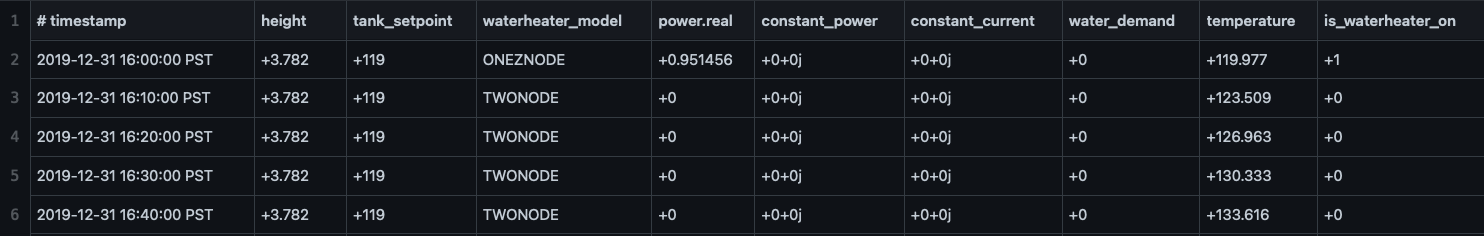
\includegraphics[width=1.1\columnwidth]{Pictures/HPWH_wrong_behavior.png}
        \caption{HPWH object in GLD does not respond to specified setpoints}
        \label{fig:HPWH}
    \end{figure}
    \begin{itemize}
        \item Comparing the HPWH behavior to the EWH, we can see the issue clearly. Figure \ref{fig:EWH} shows the EWH behavior under the same parameters.
    \end{itemize}
    \begin{figure}[htp!]
        \centering
        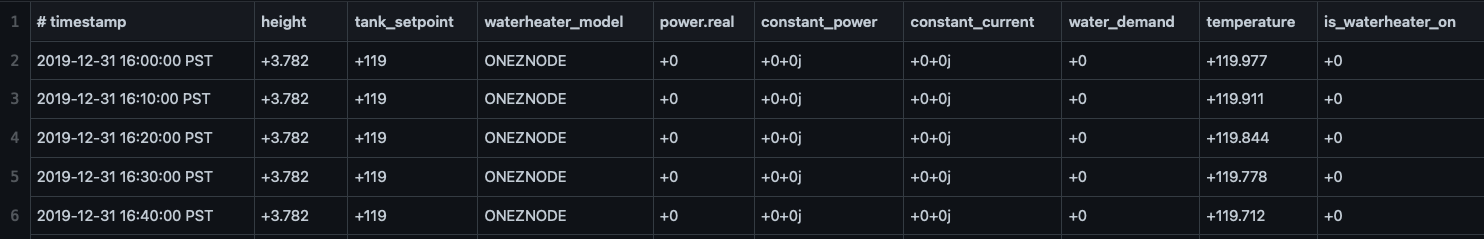
\includegraphics[width=1.1\columnwidth]{Pictures/EWH.png}
        \caption{EWH object in GLD responds properly to specified setpoints}
        \label{fig:EWH}
    \end{figure}
\newpage
    
\subsection{debugging}
\subsubsection{Related links}
\begin{itemize}
    \item Here's my conversation with Frank Tuffner, a GridLAB-D developer, regarding the HPWH. \href{https://sourceforge.net/p/gridlab-d/discussion/842562/thread/4a543d83a0/?limit=25#71e9}{Frank's input regarding HPWH issue.}
    \item On your computer, go to GLD folder $>$ residential $>$ open waterheater.cpp file.
\end{itemize}
\subsection{Water Heater Dynamic Driving Parameters}
\begin{itemize}
    \item Demand
    \begin{itemize}
        \item The higher the demand, the more quickly the thermocline drops.
    \end{itemize}
    \item Voltage
    \begin{itemize}
        \item The line voltage of the coil. The lower the voltage, the more slowly the thermocline rises.
    \end{itemize}
    \item Inlet water temperature
    \begin{itemize}
        \item The lower the inlet water temperature, the more heat needed to raise the temperature to the setpoint.
    \end{itemize}
    \item Indoor air temperature
    \begin{itemize}
        \item The higher the indoor temperature, the less heat loss through the jacket.
    \end{itemize}
\end{itemize}
\subsection{Heating Element Capacity}
The heating element capacity equation in the EWH is voltage dependant as shown in equation \ref{equ:HEC_EWH}.
\begin{equation}
    test = HeatingElementCapacity *(ActualVoltage)^2 / (NominalVoltage)^2
    \label{equ:HEC_EWH}
\end{equation}
However, the heating element capacity for the heat pump water heater does not have a voltage dependence as shown in equation \ref{equ:HEC_HPWH}.
\begin{equation}
    HeatingElementCapacity = (1.09 + (1.17 - 1.09) * (get_Tambient(location) -50) / (70 - 50)) * (0.379 + 0.00364 * Tw)
    \label{equ:HEC_HPWH}
\end{equation}

\subsection{Commented commands by GLD folks}
\begin{itemize}
    \item Heating element capacity (line 1634)
    \item Water temperature increment for onenode and twonode analysis (lines 1656 and 1684)
    \item Coesfficient of Performance (CoP) line 1731
\end{itemize}
\subsection{Water Heater Source Code Structure}
\begin{itemize}
    \item The code is defined by parameters instead of water heater models. 
    \item Some parameters, such as tank\textunderscore area, tank\textunderscore volume, tank\textunderscore height, etc are global as they work with all water heater models (i.e Electric, heat pump, and gas).
    \item Other parameters, such as heating element, need to be calculated when using Heat pump water heater model. The heating element in heat pump water heater is used as a backup.
\end{itemize}
\subsection{Errors Summary}
Running the HPWH object in GLD, we see the following errors:
\begin{itemize}
    \item The property is\textunderscore waterheater\textunderscore on is randomly 1 or 0. For a correct HPWH behavior, it should be 1 when there's sufficient water demand. Otherwise, it should always be zero.
    \item The waterheater\textunderscore model property should be ONEZNODE when there is no water demand. When there is water demand, there is inlet water pumped inside the tank. Therefore, both heating element capacity (top and bottom) should turn on. When both heating element capacity are on, the model switches to TWONODE model which is not the case in the HPWH. Refer to figure \ref{fig:EWH} and figure \ref{fig:HPWH} for a visual analysis.
\end{itemize}
\subsection{Questions}
\begin{itemize}
    \item I know the heating element is used as a backup in the HPWH. How is “backup” defined? Is it used where there’s a high water demand? How high should the water demand be to turn on the heating element?
    \begin{itemize}
        \item There are four modes in the A. O Smith units~\cite{r1}. These modes are listed as shown below:
        \begin{itemize}
            \item \textbf{Hybrid Mode:}
            \begin{itemize}
                \item This mode uses the dead-band algorithm. If the average tank temperature (the weighted temperature of the upper and lower thermostat) drops below 9F below the setpoint, then the HP turns on to heat the water.
                \item If the HP fails to heat the water to the setpoint (i.e due to high water demand.) and the average temperature drops more than 20F below the setpoint, then the upper heating element replaces the HP as the heating source. 
                \item The unit uses the HP until 75$\%$ of the available hot water has been depleted. 
            \end{itemize}
            \item \textbf{Efficiency Mode}
            \begin{itemize}
                \item This mode does not use the electric resistance elements, unless the ambient temperature is outside the safe operating range (45°–109°F) of the heat pump.
            \end{itemize}
            \item \textbf{EWH Mode}
            \begin{itemize}
                \item HPWH acts as EWH. Upper element turns ON first to heat the top of the tank and then lower element turns on to heat the bottom of the tank.
            \end{itemize}
            \item \textbf{Vacation Mode}
            \begin{itemize}
                \item Reduce the temperature setpoint (default is 60F)
            \end{itemize}
        \end{itemize}
    \end{itemize}
\end{itemize}
\subsubsection{Heating Element Operation Principle in HPWH}
The heating element operates under the following circumstances:
\begin{itemize}
    \item If the air temperature is outside the safe range (45 - 120F)
    \item If the water in the tank is significantly lower than the set point, the upper element operates. The difference between the tank temperature and the set point depends on the circumstances, but it is generally 25°–30°F.
    \item If the system senses that the water use is too high, the lower element operates. In general, 25–30 gal within a short time period is considered high water use. Once the lower electric resistance element engages, the entire tank is reheated like a traditional ERWH.
\end{itemize}
\newpage
\subsection{How does a Heat Pump Water-Heater work?}
    \begin{figure}[htp!]
        \centering
        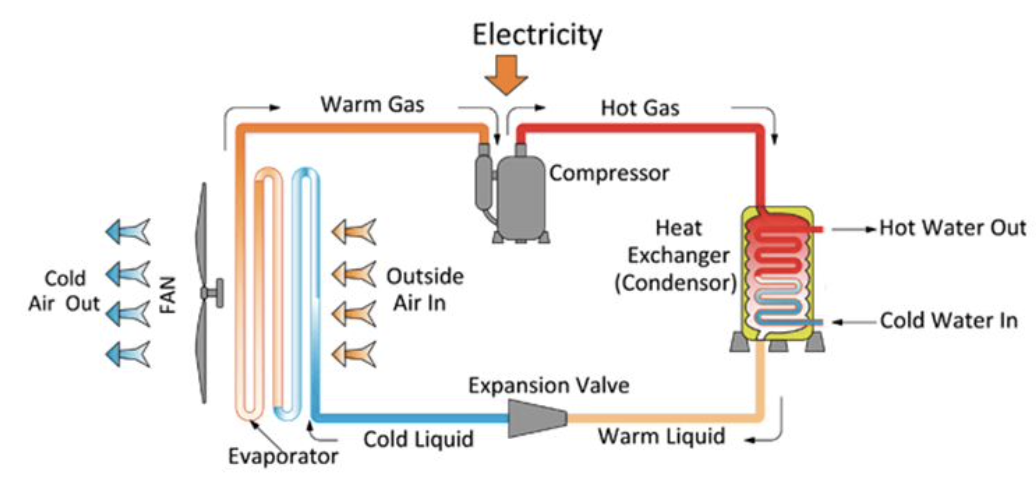
\includegraphics[width=1.1\columnwidth]{Pictures/HPWH_working_principle.png}
        \caption{source:\href{https://inukiengineering.com/heat-pump-water-heaters/}{nukiengineering.com}}
        \label{fig:EWH2}
    \end{figure}
I will start with a basic, however, very important thermodynamic principle. \textbf{HEAT ALWAYS GOES TO COLD.} Compressor increases the pressure of the gas passing through to make its temperature very high. This coil goes through the tank which heats up the water inside the tank (top portion). The heat of the gas gets released as it goes down the tank. The output of the tank is the same gas but with less hot temperature. The liquid goes through an expansion valve. The expansion valve "release" the liquid (less pressure therefore less heat) to make the liquid temperature less hot (cold). When the liquid goes through the evaporator, the temperature of the liquid is way less than the outside temperature. Therefore, the cold air gets dumped out and heat comes in. Thus, warm gas goes in to the compressor again and the same cycle is repeated.
\subsection{Coefficient of Performance (CoP)}
In EWH, we measure the efficiency to understand the performance of the WH. However, in the HPWH, we measure the CoP to see the ratio of useful heating or cooling provided to the required work as shown in equation \ref{equ:CoP}. \par
In GridLAB-D waterheater.cpp file, the CoP of the HPWH is defined with an equation that contains a set of integers. To make CoP more accessible, we need a more general equation. 
\begin{equation} \label{equ:CoP}
    CoP = \frac{E_{delivered}}{E_{in}}
\end{equation}
$E_{delivered}$ can be defined as:
\begin{equation}\label{equ:E_delivered}
    \Delta E_{delivered} = \frac{(V_{i}\rho_{w}C_{p,w}(T_{t,i}-T_{ref})) - (V_{i}\rho_{w}C_{p,w}(T_{t-1,i} - T_{ref}))}{t}
\end{equation}
Where:
\begin{itemize}
    \item $V_{i}$ = Volume of the node
    \item $\rho_{w}$ = water density of the node
    \item $C_{p,w}$ = water specific heat capacity.
    \item $T_{t,i}$ = Temperature of the node measured at time t.
    \item $T_{ref}$ = reference water temperature (default)
    \begin{itemize}
        \item For inlet water, the temperature is 60 $^{\circ}$.
    \end{itemize}
\end{itemize}
\newpage

